
Dada la siguiente topología:

\begin{itemize}
  \item La máquina UML1 realiza un anuncio de prefijos, y es la única
  autorizada
  \item La máquina UML3 también intentará hacerlo, pero OpenFlow lo impedirá
\end{itemize}

\begin{figure}[h]
  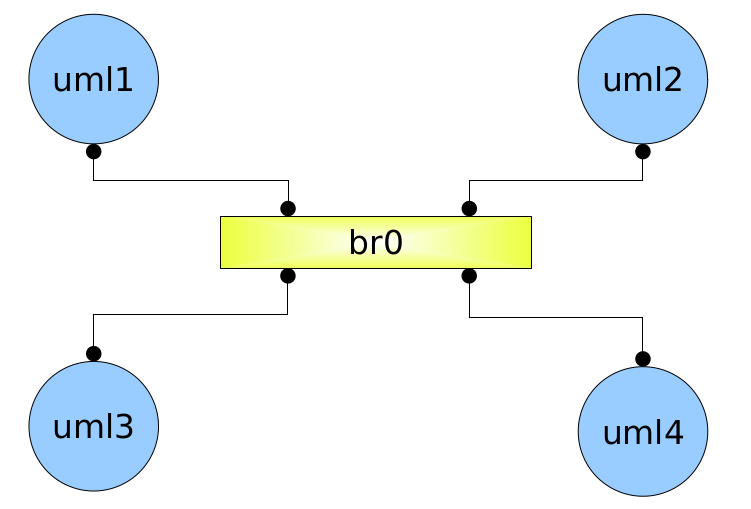
\includegraphics[width=\textwidth]{ovs-ofctl.png}
  \centering
\end{figure}

Anuncios de prefijos:

\begin{itemize}
  \item UML1: 2001:db8:1::/64
  \item UML3: 2001:db8:3::/64
\end{itemize}

\begin{minted}{bash}
  # net.conf
  defsw br0 uml1.0 uml2.0 uml3.0 uml4.0
\end{minted}

\begin{minted}{lexer.py:IOSLexer -x}
  ! UML1
  con[figure] t[erminal]
  int eth0
  no [shutdown]
  ipv6 nd prefix 2001:db8:1::/64
  no ipv6 nd suppres-ra
  q[uit]
  ipv6 f[orwarding]
  end
  w[rite]
\end{minted}

\begin{minted}{lexer.py:IOSLexer -x}
  ! UML1
  con[figure] t[erminal]
  int eth0
  no [shutdown]
  ipv6 nd prefix 2001:db8:3::/64
  no ipv6 nd suppres-ra
  q[uit]
  ipv6 f[orwarding]
  end
  w[rite]
\end{minted}

\begin{minted}{lexer.py:IOSLexer -x}
  ! UML2 y UML4
  con[figure] t[erminal]
  int eth0
  no [shutdown]
  end
  w[rite]
\end{minted}

En este momento, tanto UML1 como UML3 están anunciando sus prefijos.
La manera de comprobarlo es ejecutar el comando \mintinline{bash}{ifconfig}
en UML2 y UML4, como se muestra a continuación:

\begin{minted}
  [
    frame=lines,
    framesep=2mm,
    baselinestretch=1.2,
    bgcolor=LightGray,
    fontsize=\footnotesize
  ]
  {bash}
  root@uml2:~# ifconfig
  eth0    Link encap:Ethernet  HWaddr 02:00:00:00:02:f0
          inet6 addr: 2001:db8:3::ff:fe00:2f0/64 Scope:Global
          inet6 addr: fe80::ff:fe00:2f0/64 Scope:Link
          inet6 addr: 2001:db8:1::ff:fe00:2f0/64 Scope:Global
          UP BROADCAST RUNNING MULTICAST  MTU:1500  Metric:1
          RX packets:59 errors:0 dropped:0 overruns:0 frame:0
          TX packets:9 errors:0 dropped:0 overruns:0 carrier:0
          collisions:0 txqueuelen:1000
          RX bytes:6589 (6.4 KiB)  TX bytes:734 (734.0 B)
          Interrupt:5

  lo      Link encap:Local Loopback
          inet addr:127.0.0.1  Mask:255.0.0.0
          inet6 addr: ::1/128 Scope:Host
          UP LOOPBACK RUNNING  MTU:65536  Metric:1
          RX packets:4 errors:0 dropped:0 overruns:0 frame:0
          TX packets:4 errors:0 dropped:0 overruns:0 carrier:0
          collisions:0 txqueuelen:0
          RX bytes:200 (200.0 B)  TX bytes:200 (200.0 B)
  root@uml2:~#
\end{minted}

\newpage

En el shell maestro debemos ejecutar las siguientes líneas:

\begin{minted}{bash}
  redes@RED:~$ sudo su
  # Borrar los posibles flujos que puedan existir sobre br0
  redes@RED:~# ovs-ofctl del-flows br0
  # Añadir un flujo a br0 que dropee los mensajes ICMPv6 del tipo
  # ROUTER_ADVERTISEMENT que provengan de UML3
  redes@RED:~# ovs-ofctl  add-flow br0 "table=0, priority=200 \
  > ipv6_src=fe80::ff:fe00:3f0/128 icmp6 icmp_type=134 actions=drop"
  redes@RED:~#
\end{minted}

Una vez hecho esto, podemos comprobar apagando la int \texttt{eth0} de UML2
o UML4 y volviendo a levantar, que ahora los anuncios de UML3 están restringidos,
y por tanto, no llegarán anuncios a través del bridge:

\begin{minted}
  [
    frame=lines,
    framesep=2mm,
    baselinestretch=1.2,
    bgcolor=LightGray,
    fontsize=\footnotesize
  ]
  {bash}
  root@uml2:~# ifconfig
  eth0    Link encap:Ethernet  HWaddr 02:00:00:00:02:f0
          inet6 addr: fe80::ff:fe00:2f0/64 Scope:Link
          inet6 addr: 2001:db8:1::ff:fe00:2f0/64 Scope:Global
          UP BROADCAST RUNNING MULTICAST  MTU:1500  Metric:1
          RX packets:61 errors:0 dropped:0 overruns:0 frame:0
          TX packets:17 errors:0 dropped:0 overruns:0 carrier:0
          collisions:0 txqueuelen:1000
          RX bytes:6781 (6.6 KiB)  TX bytes:1390 (1.3 KiB)
          Interrupt:5

  lo      Link encap:Local Loopback
          inet addr:127.0.0.1  Mask:255.0.0.0
          inet6 addr: ::1/128 Scope:Host
          UP LOOPBACK RUNNING  MTU:65536  Metric:1
          RX packets:4 errors:0 dropped:0 overruns:0 frame:0
          TX packets:4 errors:0 dropped:0 overruns:0 carrier:0
          collisions:0 txqueuelen:0
          RX bytes:200 (200.0 B)  TX bytes:200 (200.0 B)
  root@uml2:~#
\end{minted}


